%% Method overview figure (one column). Graphic: figures/method.png
%% The three panels and their (a)/(b)/(c) labels are baked into the image itself,
%% so this file is a single \includegraphics rather than three stacked ones.
%%   (a) DINOv3 retrieval from the pool of reference touches, with cosine similarity bars
%%   (b) coarse alignment by local feature matching, homography, and warping
%%   (c) learning-based refinement of the initial transfer
\begin{figure}[t]
  \centering
  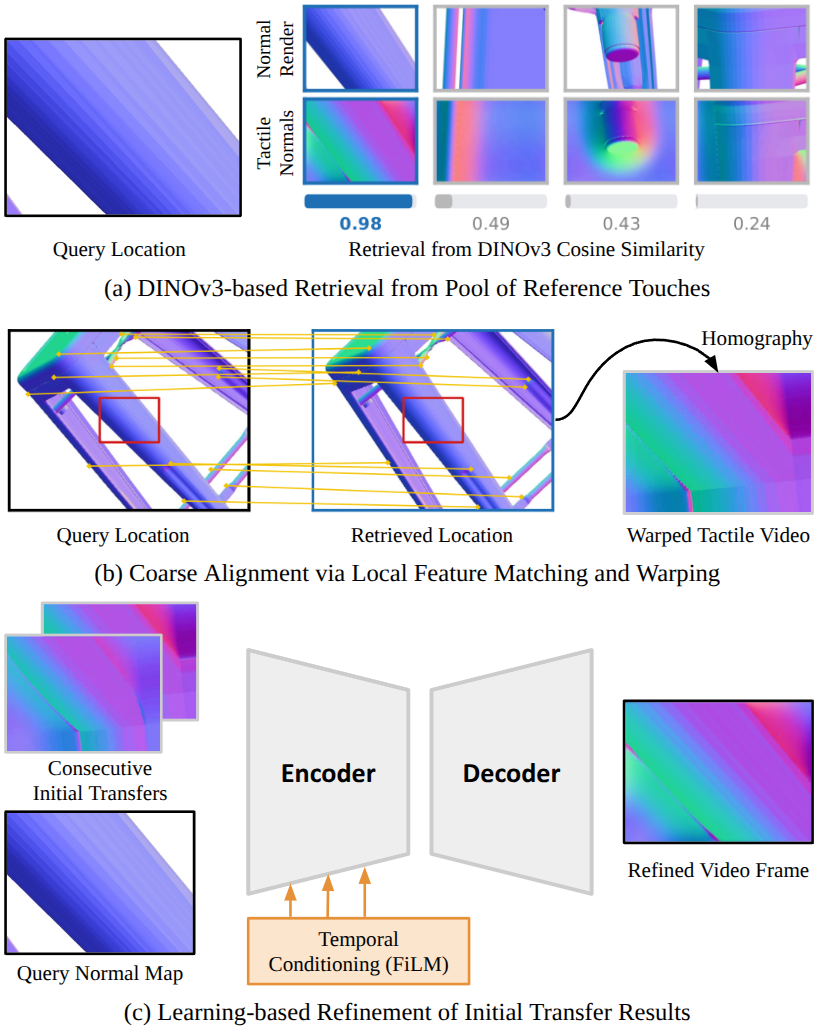
\includegraphics[width=\linewidth]{figures/method.png}
  \caption{\textbf{Method overview.} \emph{(a)} Every reference touch is stored alongside a
    surface normal render at its sensor pose, shown above its tactile normals. We encode the
    normal renders with a frozen DINOv3 encoder and score each reference against the query by
    cosine similarity, shown as the bar under each candidate, then keep the top-1 match
    (Sec.~\ref{sec:retrieval}). \emph{(b)} We match local features between the query normal render
    and the retrieved one, drawn here as yellow correspondences, and fit a homography to them. The
    homography warps the retrieved tactile video into the query frame to give the initial transfer
    (Sec.~\ref{sec:coarse}). The red box marks the patch the sensor itself covers inside the wider
    render. \emph{(c)} A lightweight encoder-decoder network refines the initial transfer. It
    receives a pair of consecutive initially transferred frames together with the query normal
    map, which tells it the surface geometry it is predicting for, and the normalized timestamp of
    the frame enters through feature-wise linear modulation (FiLM) so that the network knows where
    in the press it is (Sec.~\ref{sec:refine}).}
  \label{fig:method}
\end{figure}
